\subsection*{Control persists near the boundary, but the boundary is not crossed}

We next moved the target from the actual training maximum (Q80 boundary) through Q85, Q90 and Q95. Continuous conditioning remained operational in every matched cell, with validity between 0.56 and 0.584 and strict-hit rates between 0.522 and 0.570. Binary conditioning remained usable at the boundary and Q85, but its fixed threshold became single-class after Q80 truncation; all five Q90 and Q95 cells were therefore unsupported rather than silently treated as zero-quality successes.

\begin{figure}[H]
\centering
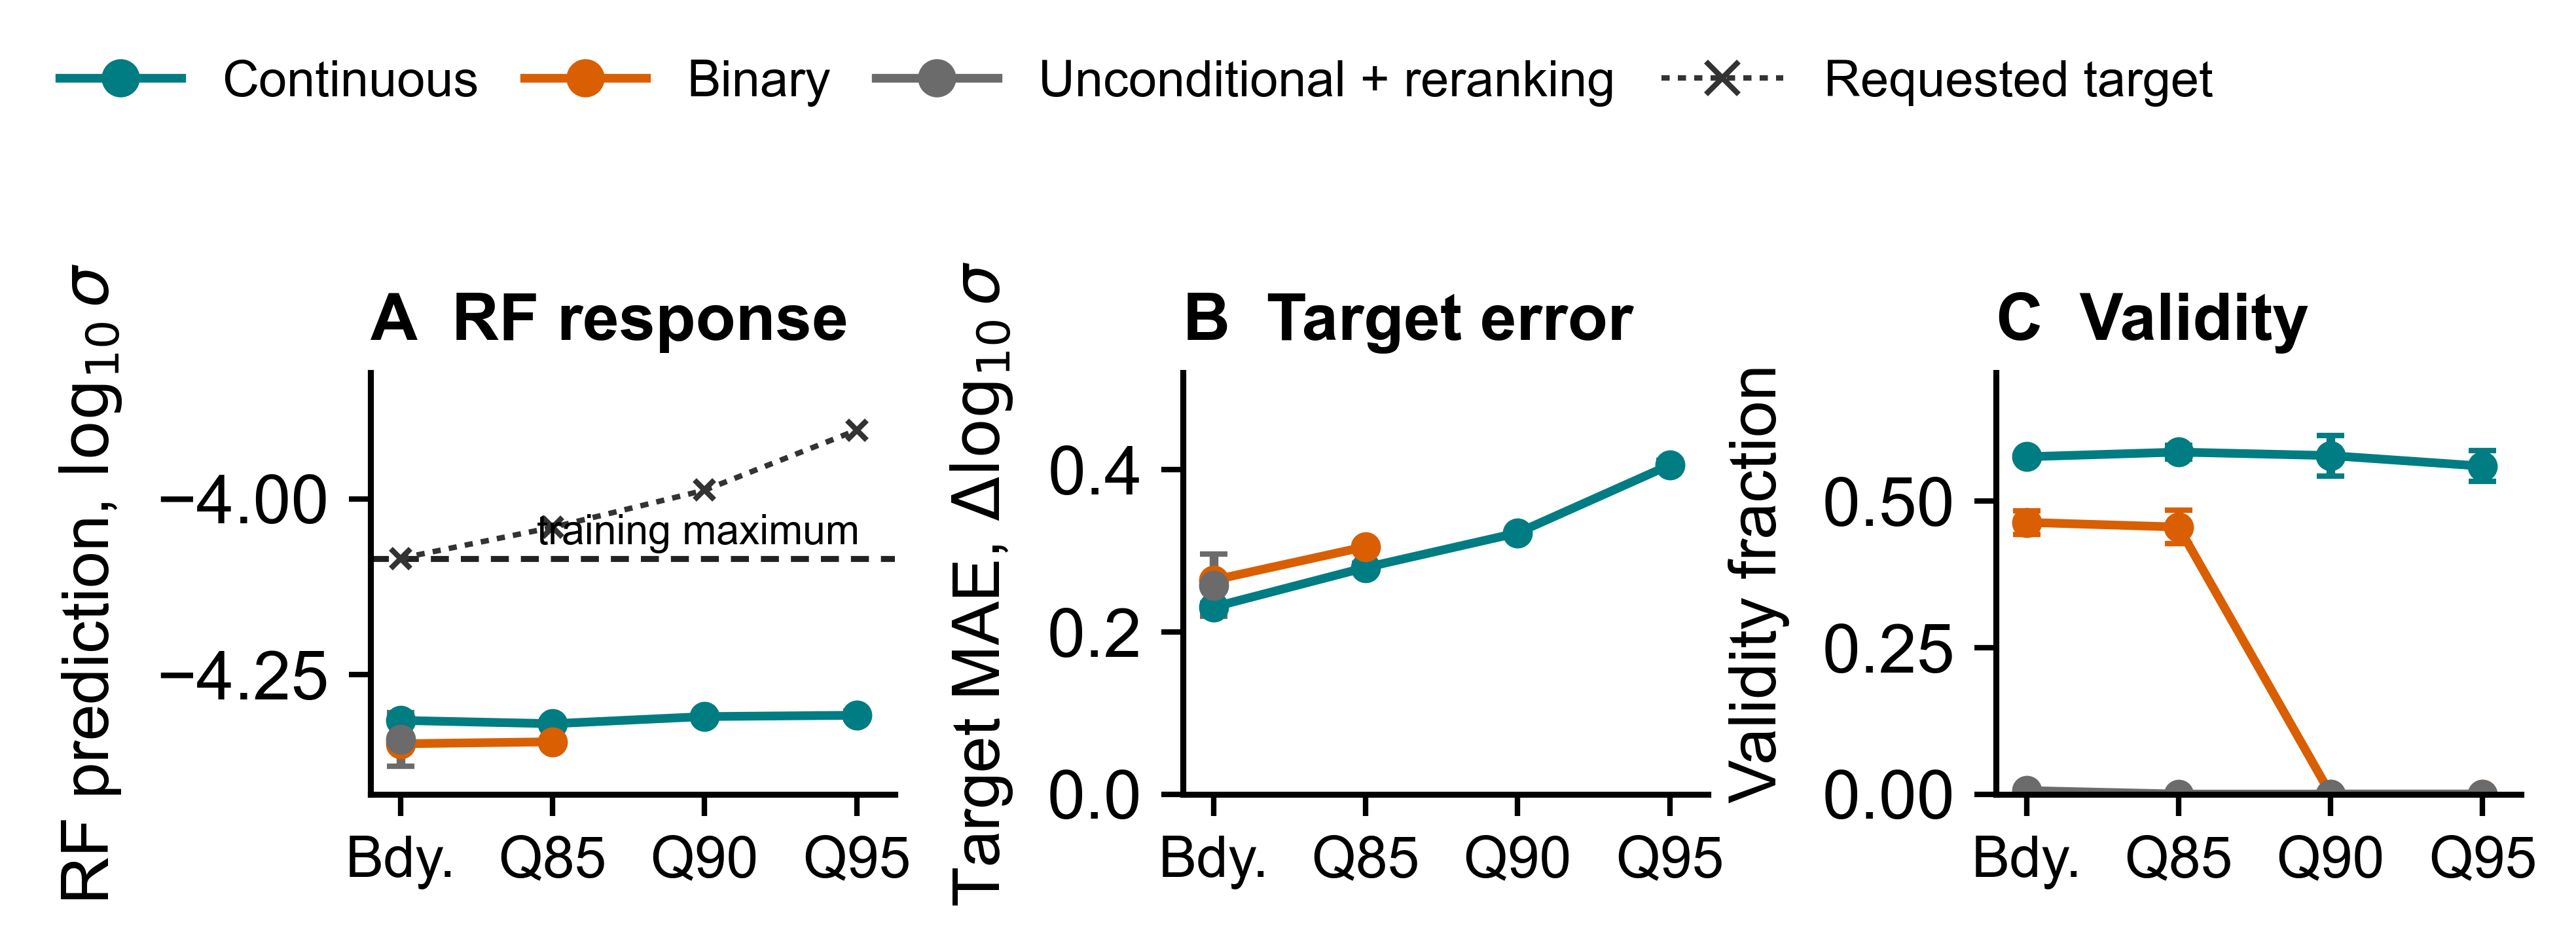
\includegraphics[width=0.98\linewidth]{figures/Figure_1_upper_tail_response.png}
\caption{Upper-tail response. Continuous conditioning degrades gradually as the target approaches the training frontier; binary conditioning becomes structurally unsupported when its fixed threshold cannot encode the requested region.}
\label{fig:upper-tail-response}
\end{figure}

The RF predictions also remained below the requested targets in this regime: the upper-tail predicted-hit rate was 0.0 for every arm and query in the locked audit. Thus the upper-tail experiment measures boundary approach and support degradation, not successful extrapolation. This distinction motivates the next benchmark.
